% 
% Annual Cognitive Science Conference
% Sample LaTeX Paper -- Proceedings Format
% 

% Original : Ashwin Ram (ashwin@cc.gatech.edu)       04/01/1994
% Modified : Johanna Moore (jmoore@cs.pitt.edu)      03/17/1995
% Modified : David Noelle (noelle@ucsd.edu)          03/15/1996
% Modified : Pat Langley (langley@cs.stanford.edu)   01/26/1997
% Latex2e corrections by Ramin Charles Nakisa        01/28/1997 
% Modified : Tina Eliassi-Rad (eliassi@cs.wisc.edu)  01/31/1998
% Modified : Trisha Yannuzzi (trisha@ircs.upenn.edu) 12/28/1999 (in process)
% Modified : Mary Ellen Foster (M.E.Foster@ed.ac.uk) 12/11/2000
% Modified : Ken Forbus                              01/23/2004
% Modified : Eli M. Silk (esilk@pitt.edu)            05/24/2005
% Modified : Niels Taatgen (taatgen@cmu.edu)         10/24/2006
% Modified : David Noelle (dnoelle@ucmerced.edu)     11/19/2014

%% Change "letterpaper" in the following line to "a4paper" if you must.

\documentclass[10pt,letterpaper]{article}

\usepackage{cogsci}
\usepackage{pslatex}
\usepackage[natbibapa]{apacite}
\usepackage{amsmath}
\usepackage{amssymb}
\usepackage{xcolor}  % for \todo
\usepackage{graphicx}


\title{Compositional sub-goal representations for planning and problem-solving}

\newcommand{\todo}[1]{\textcolor{red}{\textsc{[TODO: #1]}}}


\author{Anon Y. Mous}


\begin{document}

\maketitle


\begin{abstract}
When faced with a large and complex problem, people naturally break it up into several smaller and simpler problems. This hierarchical decomposition of an ultimate goal into sub-goals facilitates planning by reducing the number of factors that must be considered at one time. However, it can also lead to suboptimal decision making, leading one to miss opportunities to make progress towards multiple subgoals with a single action. This potential for suboptimality can be ameliorated by considering multiple subgoals at once, but at the cost of increasing the number of factors that must be considered and thus increasing the computational burden of planning. Here, we present a model of planning with compositional goal representations and show that it explains the errors people make in a Towers of London task better than a limited-depth search model. Our results suggest that people are capable of representing and pursuing multiple subgoals at once, but that the number of subgoals is generally quite limited. Furthermore, we find that the degree of representational limitation may be an important latent dimension for explaining individual differences in planning ability. Finally, we (hopefully!) find that the inferred representational limitations are sensitive to the cost of suboptimal planning, indicating that people may rationally choose a goal representation that trades off between representational costs and decision quality.

\textbf{Keywords:} 
planning; hierarchy; goals
\end{abstract}


\section{Introduction}

It's Tuesday afternoon and you have a list of errands to run before you can return home to watch last night's episode of \textit{The Bachelor}. You need to mail a letter, pick up broccoli for tonight's stir fry, and drop off a book at the library. You are eager to get home to see whether Hannah received one of the coveted roses, and thus want to accomplish these tasks as expediently as possible. There are two library locations, four grocery stores, and who knows how many mail boxes in your town; how do you decide which location of each to visit, and in what order? Unfortunately, you have been presented with the generalized traveling salesman problem, which is known to be NP-hard (that is, very difficult to solve). You might simplify the problem by focusing on only one errand at a time, completing it as quickly as possible from wherever the last errand left you. But by ignoring your other tasks when planning how to complete one, you might miss the opportunity to save time by going to the library location that is further from your house, but right next to a grocery store.

How might people navigate this tradeoff between complexity and efficiency? One possibility is that they choose some subset of goals and construct a plan that is optimal with respect to that subset, asking themselves, for example, "what is the fastest way to get to both a grocery store and a library?" and leaving future goals such as dropping off a letter for future consideration. In this project, we sought evidence for this kind of joint goal pursuit.

\section{Background}

\subsection{Search and its limitations}

Many of the hallmarks of higher level human cognition, such as problem solving, strategic reasoning, and planning may rely on a single core capacity: search \cite{NewellSimon1972}. \todo{}

In complex domains, exhaustive search is computationally intractable; thus search must be curtailed in some way. When extensive experience is available, people may avoid search by relying on model-free reinforcement learning \citep{Keramati2011,Kool2017} or cached action sequences \citep{Huys2015}. When rewards are dense, they may use these local signals of progress to avoid less promising branches of a decision tree \citep{Huys2012}. However, many of the problems people encounter in their daily lives lack such structure. In such cases, people may simply cut off search at some arbitrary point. The simplest version of this strategy is \textit{depth-limited search}, which (perhaps due to it's simplicity) has been incorporated into many models of human search \citep{MacGregor2001,Keramati2016,Krusche2018}. Under this strategy, the searcher considers all possible action sequences of some length $d$, and chooses the one that gives the best intermediate outcome. For reward-seeking planning, this outcome is the sum of rewards one receives along this path (and perhaps also a learned value of the final state; \citealp{Keramati2016}). In problem solving settings, there are typically no intermediate rewards, and a heuristic estimate of distance to the goal state is used to evaluate partial plans.


% \citet{Campitelli2004} show that more skilled chess players search deeper.


\subsection{Tower of London}

Tower of London (ToL), introduced in \cite{Shallice1982}, is a variant of Tower of Hanoi (ToH) designed to improve upon ToH to be a graded measure of planning and problem solving ability.  In ToL, three beads of different colors on a board with three sticks of varying lengths (thus resulting in restrictions on the number of beads that can be stacked in a position) must be moved from an initial configuration to match a target configuration.

Our variant of ToL removes restrictions on stack height, marks blocks with alphabet letters, and has a standard goal position instead of having a standard initial position. XX ? Could try to justify these choices as being about simplifying the task of goal representation to dissociate the mapping from visual cues to goal representations from the use of these goal representations in planning ; Could cite Zhang, Norman 94 XX. With these modifications to the rules, our experimental task resembles Blocks World, a domain used to investigate problem solving in artificial intelligence research XXX connect to Sussman.

Prior work (Simon1975) has established various strategies people might use when solving ToH puzzles, and other studies have even taught specific strategies to people to examine the relationship between the underlying cognitive mechanisms implicated by these strategies and measures like response time (Anderson2001) and fMRI signal (Anderson2005).

XXX probably doesn't make sense for right here, needs more intro: The Sussman anomaly exemplifies a case where acting optimally with respect to individual subgoals renders a problem impossible to complete. This issue can be avoided by changing the structure of subgoals or planning with respect to multiple subgoals. More generally, some efficiencies in problems can only be achieved by planning with respect to multiple subgoals as plans based on individual subgoals may be myopic, greedily optimizing for the subgoal at hand. For instance, Figure 1 demonstrates a case where considering a single subgoal might result in an extraneous move that is avoided when considering multiple subgoals.

\subsection{Introduce idea of limited depth planning.}

Background on hierarchical representation and subgoals.

Compositional goals/options.

Overview of present work.

\begin{figure}[ht]
    \centering
    % HACK should probably be 6cm??
    % Also should definitely add better demarcation of subgoals to this
    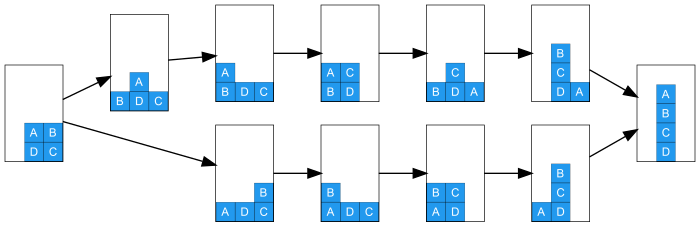
\includegraphics[width=7cm]{example-4-block}
    \caption{Planning to stack C on top of D might result in either of the two depicted plans, where A or B is first removed. Removing A first (the lower plan) winds up being more optimal, taking 1 step fewer to achieve the goal state. When planning with respect to two subgoals (stack C on top of D and stack B on top of C), an agent will always choose to remove A first since they are optimizing for the eventual placement of B.}
\end{figure}



\section{Model}
We model participant decisions as emerging from a two step hierarchical planning procedure. 

- Limited depth model

- Limited goal representation model



\section{Experiment}

\subsection{Methods}
\subsubsection{Stimuli and procedure}

In each trial, participants are presented with two configurations of stacked blocks marked with letters of the alphabet and asked to rearrange the blocks in one stack to match the blocks in the other or goal stack (Fig. XX). Only the top block of a stack can be moved, and the board is limited to contain at most 3 spaces for stacks. In all trials, the goal stack contains the same blocks arranged in alphabetical order in the middle space. Participants were asked to complete 3 tutorial trials of increasing difficulty (a 3-block trial, a 4-block trial, and a 5-block trial) and then complete 16 6-block trials which were analyzed below.
% Following the completion of the trials, participants completed a short survey to assess XXX (do we mention this?).
% Fred: No, it's to solicit feedback on the experiment, not actually part of the study.

\begin{figure}[ht]
    \centering
    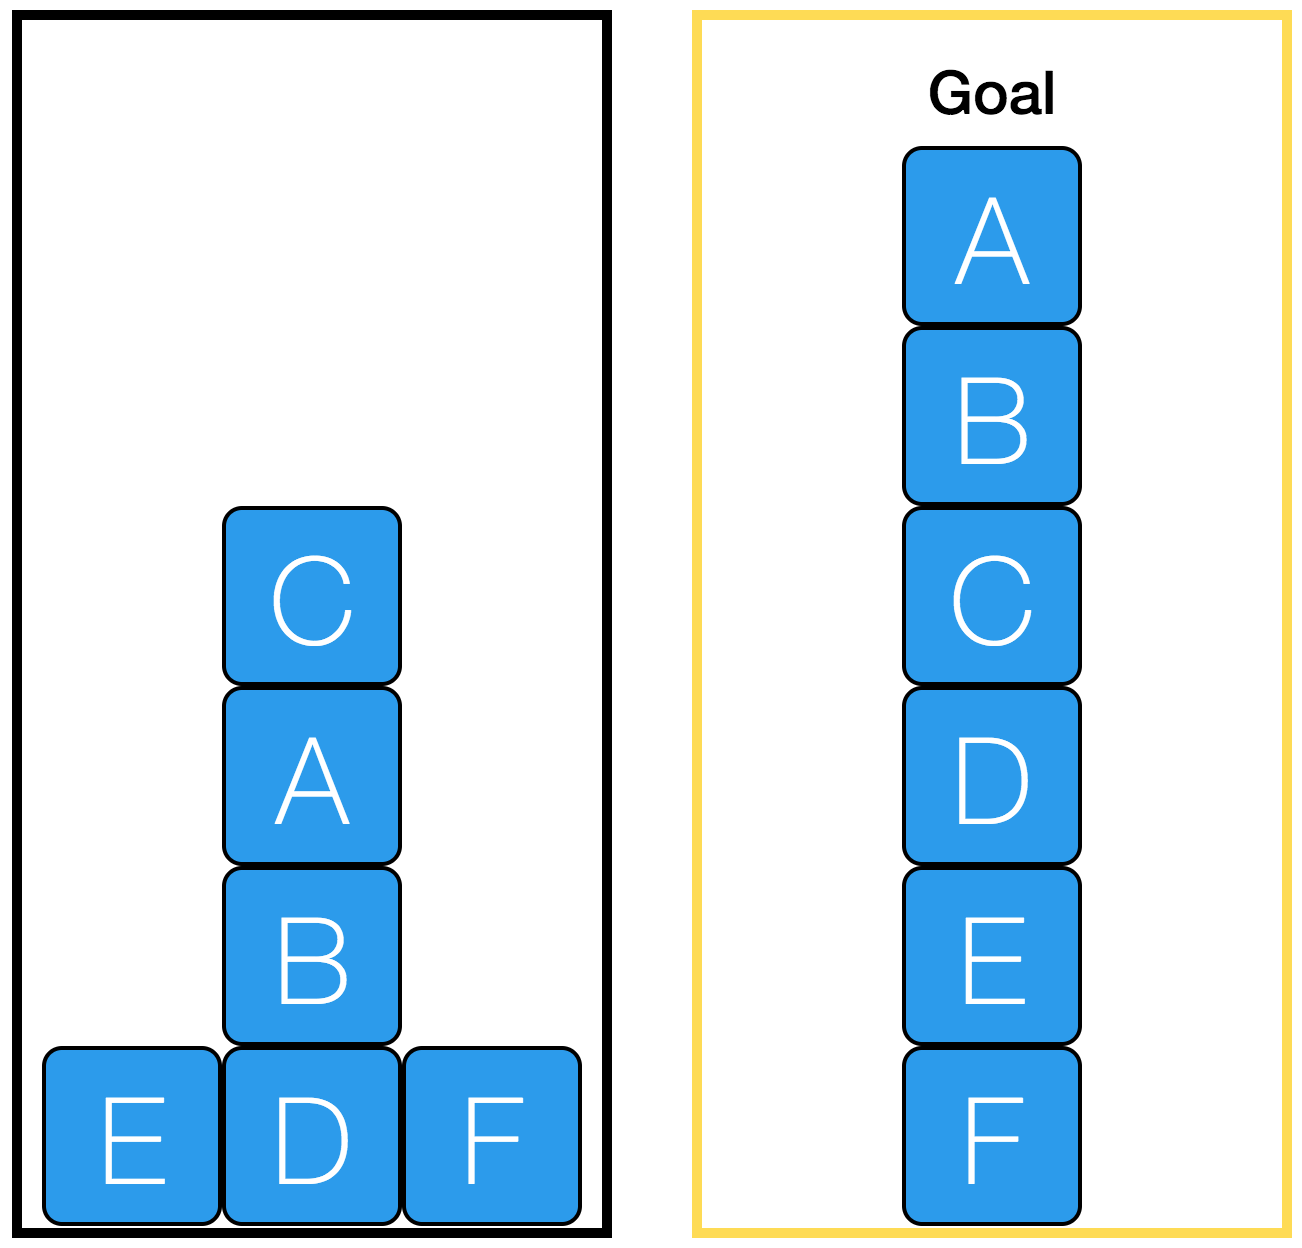
\includegraphics[width=6cm]{example-block-world}
    \caption{Interface for each trial. On the left is the initial state which must be rearranged to match the goal state at right.}
\end{figure}

\subsubsection{Participants}
We recruited 41 participants from Amazon Mechanical Turk. Each participant received \$2 for completing the task, which took an average of 8.9 minutes.

\subsection{Results}
Long section.


\section{Discussion}
Why does this matter? What are next steps?


\bibliographystyle{apacite}
\setlength{\bibleftmargin}{.125in}
\setlength{\bibindent}{-\bibleftmargin}

\bibliography{references}


\end{document}
